\documentclass{standalone}

\usepackage{graphicx}
\usepackage{tikz}
\usetikzlibrary{arrows}
\usetikzlibrary{decorations.markings}

\definecolor{purple}{RGB}{99,0,129}
\definecolor{gold}{RGB}{255,204,26}

\begin{document}

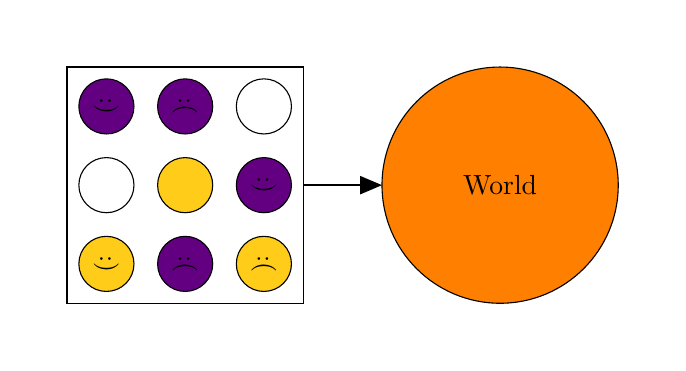
\begin{tikzpicture}

\draw[draw=none] (-0.5, -0.5) rectangle (7.5, 3.5);

\draw (0, 0) rectangle (3, 3);

\draw[fill=gold] (0.5, 0.5) circle (0.35) node[rotate=270] {\small{:)}};
\draw[fill=purple] (1.5, 0.5) circle (0.35) node[rotate=270] {\small{:(}};
\draw[fill=gold] (2.5, 0.5) circle (0.35) node[rotate=270] {\small{:(}};
\draw[fill=white] (0.5, 1.5) circle (0.35) node[rotate=270] {};
\draw[fill=gold] (1.5, 1.5) circle (0.35) node[rotate=270] {};
\draw[fill=purple] (2.5, 1.5) circle (0.35) node[rotate=270] {\small{:)}};
\draw[fill=purple] (0.5, 2.5) circle (0.35) node[rotate=270] {\small{:)}};
\draw[fill=purple] (1.5, 2.5) circle (0.35) node[rotate=270] {\small{:(}};
\draw[fill=white] (2.5, 2.5) circle (0.35) node[rotate=270] {};

\draw[fill=orange] (5.5, 1.5) circle (1.5) node {World};

\draw[thick, -triangle 45] (3, 1.5) -- (4, 1.5);

% \draw[->] (0.8, 1.8) -- (1.2, 1.8);
% \draw[<-] (0.8, 1.2) -- (1.2, 1.2);

\end{tikzpicture}

\end{document}
